% !TEX root =  ../main.tex
\section{Approach}
\label{sec:approach}

\subsection{Problem Formulation and Approach Overview} We formulate the problem as follows. Let the \textit{state} of an application at a particular point in the program be defined as a set of (variable, value) pairs $V = \{(v_1, a_1), (v_2, a_2), ..., (v_n, a_n)\}$ visible at that point during execution. 
To successfully launch an exploit on a specific \textit{sink}, an attacker needs to induce a state of the attacker's choosing at that sink. We denote this state by \textit{exploit state} and represent it with a set of (variable, value) pairs $V_E = \{(v_{e1}, b_1) (v_{e2}, b_2) ..., (v_{em}, b_m)\}$, where the variables $v_{ei}$ represent the parameters of the sink statement. Furthermore, to be able to induce state $V_E$ at the sink, the attacker can only use the input state at the \textit{source} statements defined as a set of (variable, value) pairs $V_I = \{(v_{i1}, c_1), (v_{i2}, c_2) ..., (v_{in}, c_n)\}$. 

From a defensive and application vetting perspective, there can be many sink statements of interest to an attacker and they can be located anywhere inside the application. In addition, there can be many exploits for each sink statement. For example, if an attacker has control over the application state at a database query statement, there can be many exploit states $V_E$ at his disposal, each performing a different type of SQL injection. 

% \begin{enumerate}
% 	\item \emph{Ubiquity and number of sinks}. In general, there can be many sink statements of interest to an attacker in an application and they can be located anywhere inside that application. Thus, a robust method for identifying vulnerabilities must conservatively consider every point in the program as a possible \textit{sink} statement, even though in reality attackers are more likely prone to target only a certain type of statements.
% 	\item \emph{Type of exploits}. In general, there can be many possible exploit states $V_E$ for each sink statement. Consider for example a statement that creates a query to a local database. If an attacker has control over the application state at that  statement, there can be many exploit states $V_E$ at his disposal, each of which performs a different type of SQL injection. 
% 	Thus, a robust method for identifying vulnerabilities must not rely on assumptions about specific exploit states but must easily account for any possible exploit state $V_E$ at any point in the program.
% \end{enumerate}

 Therefore, we state the problem as follows. Given a point $p$ in the program and an arbitrary exploit state $V_E$ in $p$, can we automatically determine if there exists a state $V_I$ at the \textit{source} statements that induces $V_E$ in $p$ when the program executes?  To answer this question, the relationship between the state at any point in the program and state $V_I$ at the source statements must be made explicit. The discovery of such relationship and its modeling as a function $F$, such that we can automatically compute $V_I = F(V_E)$ is at the core of our approach. The steps of our approach are described next. 

\textbf{Paths computation}. Since every program point $p$ may be a sink statement, in this first step we compute all the paths between the \textit{source} statements and every point in the program. Such analysis faces two main challenges. The first challenge arises due to the interprocedural nature of Android programs. In fact, the analysis must be able to deal with interprocedural data-flows and identify paths through deep sequences of method calls as well as recursive method calls. The second challenge is that of \textit{path explosion}, which is a common problem in data flow analysis, and which becomes even more problematic in an interprocedural context. 

To deal with these challenges, we first divide the methods into two sets: user-defined and libraries. Next, a control-flow supergraph of the user-defined methods is created by the data-flow analysis framework. In this supergraph, the call sites are joined with callee definitions and callees' exit sites are joined back with the call sites. We show a portion of the supergraph built for our example in Figure~\ref{fig:supergraph}, where each node corresponds to a statement and is labeled with the line number from code listing \ref{lst:example}. To further limit the size of the supergraph, we perform a preliminary \textit{taint propagation} step. During this step, the nodes of the supergraph are partitioned into two sets, namely the set of statements that use values in $V_I$ and can thus be influenced by an attacker, and the set of statements whose execution is independent from an attacker. 

The taint propagation and the path computation steps are modeled as an IFDS data-flow analysis problem where taint and path information is collected inside facts associated with each point in the program~\cite{heros,Bodden:2012:IDA:2259051.2259052}. 
\setlength{\belowcaptionskip}{-10pt}
\begin{figure*}[t]
  \centering
    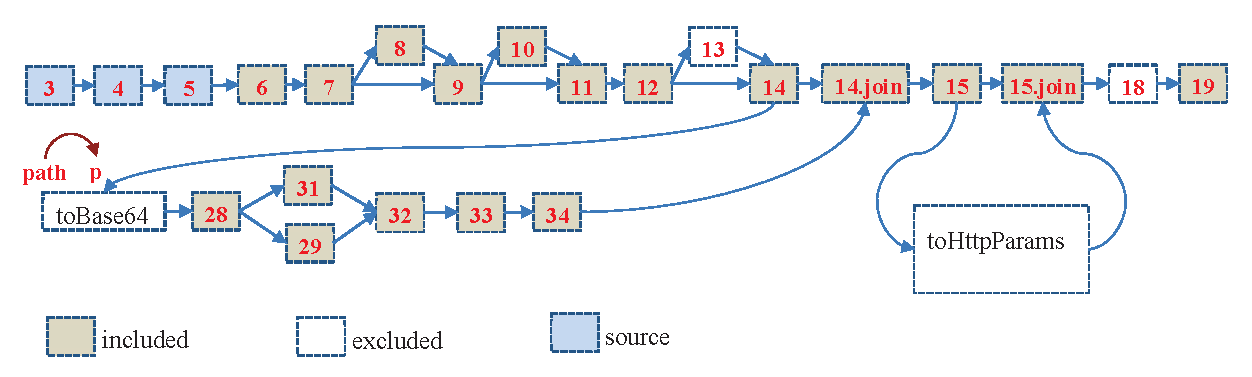
\includegraphics[width=4in]{./images/supergraph.eps}
  \caption{Supergraph built by the analysis framework. \label{fig:supergraph}}
 \end{figure*}

\textbf{Symbolic execution}. After the path computation step, symbolic execution over the paths is performed to derive the set of constraints imposed over the variable values along those paths. At the end of this step, for every program point $p$, a logic formula $F_p$ is created, whose variables correspond to program variables and whose terms correspond to the program statements that modify those variables. Thus, $F_p$ represents the relationship between the input state $V_I$ and the application state in $p$.
The syntax of the symbolic formulas used in our approach is described by the pseudo-grammar shown in Figure \ref{fig:grammar}, where terminal symbols are represented in bold. \\
\vspace{-8pt}
\setlength{\belowcaptionskip}{-5pt}
\begin{figure}[h]
  \centering
		\begin{tabular}{lll}
			$F_p$  & $\rightarrow$ & $F_{p} \vee conj \ \vert \ conj$ \\
			$conj$ & $\rightarrow$ & $(conj \wedge term)\ \vert\ term$ \\
			$term$ & $\rightarrow$ & $stat\ \vert\ \neg stat$ \\
			$stat$ & $\rightarrow$ & $statement\ \vert\ \boldsymbol{var} == statement$ \\
			$statement$ & $\rightarrow$ & $statement\ \boldsymbol{+}\ single\_stat\ \vert\ single\_stat$ \\
			$single\_stat$ & $\rightarrow$ & $\boldsymbol{var}\ \vert\ \boldsymbol{constant}\ \vert\ library\_method$ \\
			$library\_method$ & $\rightarrow$ & $\boldsymbol{solv\_stat}\ \vert\ \boldsymbol{nonsolv\_stat}$ \\
		\end{tabular}
  	\caption{Grammar of Symbolic Formula}
	\label{fig:grammar}
 \end{figure}


In particular, the terminal symbol $solv\_stat$ represent Java statements whose operations semantics can be modeled by the solver used in the exploit generation step. In addition, these are the statements that use at least one tainted variable. Conversely, $nonsolv\_stat$ represents statements that cannot be modeled by the solver. Finally, $var$ represents tainted variables, $constant$ represents constant strings, while the $+$ terminal represents string concatenation. For instance, the formula $F_p$ related to the sink statement on line 20 of Figure \ref{lst:example} is derived as:

\scriptsize
($host.contains("example.com") \wedge url$$==$$"http$://$"+host+"/"$)$\bigvee$ \\
(! $host.contains("example.com") \wedge url$$==$$"http$://$www.example.com/"$)
\normalsize
We note that each term in the symbolic formula represents a statement along the path, while each new path created by a branching statements is represented using a disjunction. Assignment operations in the code are modeled using equality constraints, in order to capture the equality conditions between two expressions. 

\textbf{Exploit generation}. The input to this step is a program point $p$, the corresponding formula $F_p$ and a set of assignments representing the exploit state $V_E$. The first operation of this step is the translation of the symbolic formula $F_p$ into the solver's language. 
In particular, for each member of the $solv\_stat$ statements, we create a set of constraints in the language of the solver, which model the behavior of that statement. The members of the $unsolv\_stat$ statements are modeled with a particular operator in the solver's language that returns the whole domain of values for the variable. 

For the implementation of this step, we chose the Kaluza solver, which provides string solving capabilities and several primitives that can model string operations~\cite{kaluza}. Given the symbolic formula $F_p \wedge V_E$ for a particular point $p$, the solver provides a (possibly empty) solution containing the values of the variables in $V_I$, corresponding to the malicious input.


